\documentclass[11pt,a4paper]{article}
\usepackage[utf8]{inputenc}
\usepackage[T1]{fontenc}
\usepackage{amsmath}
\usepackage[usenames,dvipsnames,svgnames,table]{xcolor}
\usepackage[normalem]{ulem}
\usepackage[left=1.00cm, right=1.00cm, top=0.40cm, bottom=0.4cm]{geometry}
\PassOptionsToPackage{defaults=hu-min}{magyar.ldf}
\usepackage[magyar]{babel}
\usepackage{framed, fancyhdr, wasysym, graphicx, multirow}

\begin{document}
\renewcommand{\labelitemi}{\textbullet}
\def\br{\\[0.1cm]}
\thispagestyle{empty}
\begin{center}
	\colorbox{lightgray}{{\large JPSMA3} \hspace{3cm} {\large Eseményvezérelt alkalmazások 2 2. beadandó} \hspace{5cm} \thepage}
\end{center}
\begin{framed}
	\begin{flushleft}
		{\large \textbf{Bauer Bence}}
		\hspace{3cm}{\large \textbf{2.Beadandó/19.Feladat}}
		\hspace{5.4cm}{\large 2018.11.10.}\br
		{\large JPSMA3}\br
		{\large bauerbence5@gmail.com}
	\end{flushleft}
\end{framed}
\section{Feladat}
Készítsünk programot, amellyel a potyogós amőba játékot lehet játszani, vagyis
az amőba azon változatát, ahol a jeleket felülről lefelé lehet beejteni a
játékmezőre. A játékmező itt is $nxn$-es tábla, és ugyanúgy X, illetve O jeleket
potyogtathatunk a mezőre. A játék akkor ér véget, ha betelik a tábla (döntetlen),
vagy valamelyik játékos kirak 4 egymás melletti jelet (vízszintesen, vagy átlósan).
A program minden lépésnél jelezze, hogy melyik játékos következik, és a tábla
egy üres mezőjére kattintva helyezhessük el a megfelelő jelet. Természetesen
csak a szabályos lépéseket engedje meg a program.
A program biztosítson lehetőséget új játék kezdésére a táblaméret megadásával
$(10 x 10, 20 x 20, 30 x 30)$, játék szüneteltetésére, valamint játék mentésére és
betöltésére. Ismerje fel, ha vége a játéknak, és jelenítse meg, melyik játékos
győzött (a táblán jelölje meg a győztes 4 karaktert). A program folyamatosan
jelezze külön-külön a két játékos gondolkodási idejét (azon idők összessége, ami
az előző játékos lépésétől a saját lépéséig tart, ezt is mentsük el és töltsük be).
\section{Elemzés}
\begin{itemize}
	\item A játékot tetszőleges méretű pályán játszhatjuk, melyet az ablak tetjén lévő
	mezővel tudunk beállítani, az "Új játék" gomb lenyomásával új játék indul az
	éppen a mezőben lévő pályamérettel.
	\item A feladatot egyablakos asztali alkalmazásként Windows Presentation Foundation grafikus felülettel
	valósítjuk meg.
	\item Az ablakon elhelyezünk egy File menüt (Mentés, Betöltés, Kilépés), Új játék
	beállítására szolgáló vezérlőt valamint egy státuszsort, mely a játékosok idejét és
	az éppen soron lévő játékost jelzi.
	\item A játéktáblát egy $nxn$-es nyomógombokból álló rács reprezentálja. Egy
	nyomógombra való kattintás hatására a kattintott mezőben megjelenik az éppen soron lévő játékos karaktere.
	\item A játék automatikusan feldob egy ablakot ha véget ért Döntetlen/Nyertes játékos
	nevével, valamint a két játékos idejével. Mentés/Betöltés esetén is dialógus ablakban
	történik a fájl kiválasztása.
	\item Felhasználói esetek:
\end{itemize}
\begin{figure}[h]
\centering
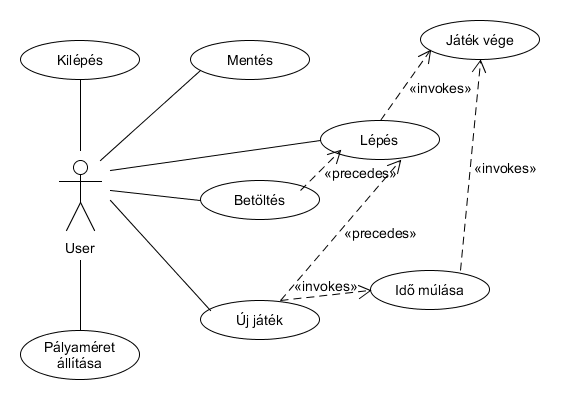
\includegraphics[width=11cm]{UMLs/UseCase.png}
\caption{Felhasználói eset diagram}
\end{figure}
\newpage
\thispagestyle{empty}
\begin{center}
\colorbox{lightgray}{{\large JPSMA3} \hspace{3cm} {\large Eseményvezérelt alkalmazások 2 1. beadandó} \hspace{5cm} \thepage}
\end{center}
\section{Tervezés}
\begin{itemize}
	\item Programszerkezet: A programot háromrétegű architektúrában valósítjuk meg:
	\begin{itemize}
		\item Megjelenítés: \textbf{View}
		\item Modell: \textbf{Model}
		\item Nézetmodell: \textbf{ViewModel}
		\item Perzisztencia: \textbf{Persistence}
	\end{itemize}
\end{itemize}
\end{document}